\documentclass[../main]{subfiles}

\questiontrue
\solutiontrue

\begin{document}
    \ifquestion
    
    \section{Quantum Star}
	
	
	
Consider a star made of degenerate matter in which the electrons of the material are in stationary states within confined regions of space. These stationary states give the electrons a certain energy associated with their quantum states.

\begin{doublespace}

    \begin{large}
        \textbf{Part A: Fermi Energy}
    \end{large}

\end{doublespace}

In this model, the electron has a wave function associated with each Cartesian axis (so it may have different wavelengths along the $x$, $y$, and $z$ axes, since it may have different momenta along each axis). From the time-independent Schrödinger equation (since we are dealing with a stationary state) for a single axis $u$, we can find the corresponding stationary wave under the confinement conditions:

\begin{equation}
-\frac{\hbar^2}{2m} \frac{d^2 \psi(u)}{du^2} + V(u)\psi = E\psi
\end{equation}

Along this axis, $u=0$ corresponds to one edge of the box, while $u=L$ corresponds to the other edge.

	\begin{figure}[htb]
		\centering
		
\tikzset{every picture/.style={line width=0.75pt}} %set default line width to 0.75pt        

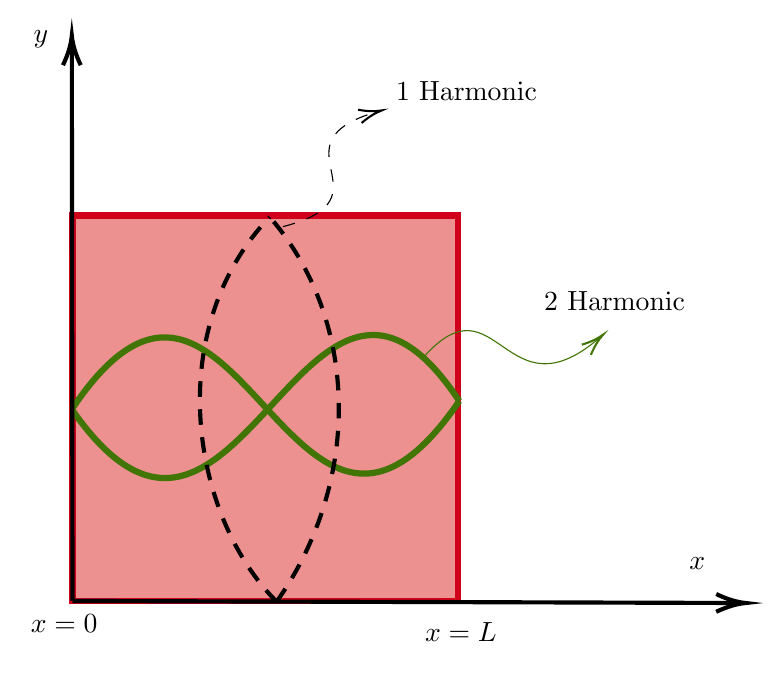
\begin{tikzpicture}[x=0.75pt,y=0.75pt,yscale=-1,xscale=1]
%uncomment if require: \path (0,408); %set diagram left start at 0, and has height of 408

%Shape: Square [id:dp44111204393396086] 
\draw  [color={rgb, 255:red, 208; green, 2; blue, 27 }  ,draw opacity=1 ][fill={rgb, 255:red, 229; green, 101; blue, 101 }  ,fill opacity=0.72 ][line width=2.25]  (197.33,140.68) -- (383,140.68) -- (383,326.34) -- (197.33,326.34) -- cycle ;
%Curve Lines [id:da7133084788617852] 
\draw [color={rgb, 255:red, 65; green, 117; blue, 5 }  ,draw opacity=1 ][line width=2.25]    (197,234.01) .. controls (276.33,115.34) and (302.33,349.34) .. (383.67,230.01) ;
%Curve Lines [id:da34226693955120857] 
\draw [color={rgb, 255:red, 65; green, 117; blue, 5 }  ,draw opacity=1 ][line width=2.25]    (197,234.01) .. controls (277,349.34) and (309,117.34) .. (383.67,230.01) ;
%Curve Lines [id:da7368053116770537] 
\draw [line width=1.5]  [dash pattern={on 5.63pt off 4.5pt}]  (295.67,326.68) .. controls (336.33,269.34) and (336,191.68) .. (292.33,141.34) ;
%Curve Lines [id:da6250150492760804] 
\draw [line width=1.5]  [dash pattern={on 5.63pt off 4.5pt}]  (295.67,326.68) .. controls (254.33,285.34) and (240.33,196.01) .. (292.33,141.34) ;
%Curve Lines [id:da6549731099708387] 
\draw [color={rgb, 255:red, 65; green, 117; blue, 5 }  ,draw opacity=1 ]   (366.67,208.68) .. controls (401.98,169.08) and (405.6,239.25) .. (451.59,199.26) ;
\draw [shift={(453,198.01)}, rotate = 137.97] [color={rgb, 255:red, 65; green, 117; blue, 5 }  ,draw opacity=1 ][line width=0.75]    (10.93,-3.29) .. controls (6.95,-1.4) and (3.31,-0.3) .. (0,0) .. controls (3.31,0.3) and (6.95,1.4) .. (10.93,3.29)   ;
%Curve Lines [id:da18419490941779104] 
\draw [color={rgb, 255:red, 0; green, 0; blue, 0 }  ,draw opacity=1 ] [dash pattern={on 4.5pt off 4.5pt}]  (298.67,146.01) .. controls (353.12,132.15) and (290.93,105.88) .. (344.67,90.47) ;
\draw [shift={(346.33,90.01)}, rotate = 164.86] [color={rgb, 255:red, 0; green, 0; blue, 0 }  ,draw opacity=1 ][line width=0.75]    (10.93,-3.29) .. controls (6.95,-1.4) and (3.31,-0.3) .. (0,0) .. controls (3.31,0.3) and (6.95,1.4) .. (10.93,3.29)   ;
%Straight Lines [id:da5083747766901023] 
\draw [line width=1.5]    (197.33,326.34) -- (518.67,327.33) ;
\draw [shift={(521.67,327.34)}, rotate = 180.18] [color={rgb, 255:red, 0; green, 0; blue, 0 }  ][line width=1.5]    (14.21,-4.28) .. controls (9.04,-1.82) and (4.3,-0.39) .. (0,0) .. controls (4.3,0.39) and (9.04,1.82) .. (14.21,4.28)   ;
%Straight Lines [id:da4146155563373559] 
\draw [line width=1.5]    (197.33,326.34) -- (197,57.01) ;
\draw [shift={(197,54.01)}, rotate = 89.93] [color={rgb, 255:red, 0; green, 0; blue, 0 }  ][line width=1.5]    (14.21,-4.28) .. controls (9.04,-1.82) and (4.3,-0.39) .. (0,0) .. controls (4.3,0.39) and (9.04,1.82) .. (14.21,4.28)   ;

% Text Node
\draw (352,74.68) node [anchor=north west][inner sep=0.75pt]   [align=left] {1 Harmonic};
% Text Node
\draw (423.33,176.01) node [anchor=north west][inner sep=0.75pt]   [align=left] {2 Harmonic};
% Text Node
\draw (177.33,50.41) node [anchor=north west][inner sep=0.75pt]    {$y$};
% Text Node
\draw (493.33,304.41) node [anchor=north west][inner sep=0.75pt]    {$x$};
% Text Node
\draw (176,331.74) node [anchor=north west][inner sep=0.75pt]    {$x=0$};
% Text Node
\draw (366,335.74) node [anchor=north west][inner sep=0.75pt]    {$x=L$};


\end{tikzpicture}
	
\caption{Example of two-dimensional arrangement}
\label{quantum}
\end{figure}

\ut{A.1} Considering that the potential inside the box of side $L$ is $V(u)=0$, prove that:

$$\psi(u)=A\sin{\left(\sqrt{\frac{2mE}{\hbar^2}}u\right)}+B\cos{\left(\sqrt{\frac{2mE}{\hbar^2}}u\right)}$$

\ut{A.2} Argue why $B=0$ is necessary.

\ut{A.3} From the wave equation: $\sqrt{\dfrac{2mE}{\hbar^2}}=\dfrac{2 \pi}{\lambda_u}$, where $\lambda_u$ is the wavelength associated with the particle along axis $u$. Argue that:

$$E=\frac{\hbar^2\pi^2}{2m^2L^2}n_u^2$$

where $n_u$ is a positive integer characterizing the quantum state of the particle.

\ut{A.4} Show that the total energy of the system is of the form:

$$E(r)=\frac{\hbar^2\pi^2}{2mL^2}r^2$$

where $r = \sqrt{n_x^2+n_y^2+n_z^2}$.

\ut{A.5} Define $N$ as the number of electrons with energy less than $E(r)$. Show that:

$$N=\frac{\pi r^3}{3}$$

\ut{A.6} Find the function $E(N)$ and integrate it from $0$ to $N_t$, the total number of particles in the star, with respect to $N$. Show that:

$$E=\frac{3\hbar^2}{10m}\left(3\pi^2\eta \right)^{\frac{2}{3}}N_t$$

where $\eta$ is the particle number density in the region.

\begin{doublespace}

    \begin{large}
        \textbf{Part B: Gravitational Self-Potential Energy}
    \end{large}

\end{doublespace}

\ut{B.1} Consider a sphere of mass and initial radius $m$ and $r$. Calculate the work required to add an incremental mass $dm$ to this sphere. Show that the increase in the system's potential energy is:

$$dE=-\frac{Gm}{r}dm$$

\ut{B.2} Relating $m$ and $r$ for a sphere of constant density $\rho$ and integrating, show that the total potential energy of the final system is:

$$E=-\frac{3}{5}\frac{GM^2}{R}$$

\begin{doublespace}

    \begin{large}
        \textbf{Part C: Degenerate Stellar Remnants}
    \end{large}

\end{doublespace}

\ut{C.1} Find the total energy of a white dwarf of mass $M$ and radius $R$, composed of an element $X$ with atomic number $Z$ and atomic mass $m_X$ (mass of one atom). Consider that other energy contributions, apart from gravitational, electron energy, and rest energy, are negligible.

\ut{C.2} Given a mass $M$, find the radius of the white dwarf associated with this mass. Show that this value is:

$$R=\frac{\hbar^2}{Gm_e}\left(\frac{9\pi}{4}\right)^{\frac{2}{3}}\left(\frac{Z}{m_X}\right)^{\frac{5}{3}}M^{-\frac{1}{3}}$$

where $m_e$ is the electron mass.

\ut{C.3} Find the radius of a white dwarf composed of hydrogen with the mass of the Sun.
	
    \clearpage
    
    
    \fi
    
    \ifsolution
    
\section{Quantum Star}

\begin{doublespace}

    \begin{large}
        \textbf{Part A: Fermi Energy}
    \end{large}

\end{doublespace}

\ut{A.1} Notice that $0 \le u \le L$ since the particle is confined within this region. Therefore, $\psi(u) = 0$ for $u \le 0$ and $u \ge L$. Inside the imposed interval, we have:

$$-\frac{\hbar^2}{2m}\frac{d^2\psi(u)}{du^2}=E\psi$$

$$\frac{d^2\psi(u)}{du^2}=-\frac{2mE}{\hbar^2}\psi$$

Solving this differential equation (which resembles a simple harmonic motion equation), we find:

$$\psi(u)=A\sin{\left(\sqrt{\frac{2mE}{\hbar^2}}u\right)}+B\cos{\left(\sqrt{\frac{2mE}{\hbar^2}}u\right)}$$

\ut{A.2} As mentioned before, at $u=0$ there is a "node" of the particle's wavefunction, similar to the boundary condition of a stationary wave on a string. Therefore, $\psi(0)=0$. This condition is only satisfied if $B=0$, since $\cos(0)=1$.

\ut{A.3} Similarly: $\psi(L)=0$ represents the other "node." To make the sine function zero at this point, the argument must be a multiple of $\pi$:

$$\sqrt{\frac{2mE}{\hbar^2}}L=n_u\pi$$

From which we obtain:

$$E=\frac{\hbar^2\pi^2}{2m^2L^2}n_u^2$$

\ut{A.4} To find the total energy of the particle, we must consider the energy associated with its oscillatory motion along each axis. Therefore, we sum the energies for each axis: $\sum n_u^2 = n_x^2+n_y^2+n_z^2$.

\ut{A.5} To count all particles with energy less than $E(R)$, we count how many have $r<R$. This can be visualized as counting how many particles have coordinates $(n_x,n_y,n_z)$ inside a sphere of radius $R$ in this space, ensuring $\sqrt{n_x^2+n_y^2+n_z^2}<R$.

However, we are only concerned with one eighth of the sphere: the part containing all positive values (positive and negative $n$ correspond to the same state). Each electron also has a fourth quantum number (spin), so at most two electrons can occupy the same position without violating the Pauli exclusion principle:

$$N=2\frac{1}{8}\frac{4\pi R^3}{3}=\frac{\pi R^3}{3}$$

\ut{A.6} Substituting this into (A.4):

$$E(N)=\frac{\hbar^2\pi^2}{2mL^2}\left(\frac{3N}{\pi}\right)^\frac{2}{3}$$

This expression gives the energy of a single particle. To find the total energy of the system, multiply by the number of particles with that energy and integrate from $0$ to $N_t$:

$$dE(N)=\frac{\hbar^2\pi^2}{2mL^2}\left(\frac{3N}{\pi}\right)^\frac{2}{3}dN$$

Integrating gives:

$$
E=\frac{3\hbar^2}{10m}\left(3\pi^2\eta \right)^{\frac{2}{3}}N_t
$$

with $\eta=\dfrac{N_t}{L^3}$.

\begin{doublespace}

    \begin{large}
        \textbf{Part B: Gravitational Self-Potential Energy}
    \end{large}

\end{doublespace}

\ut{B.1} The work required to add this incremental mass is the change in potential energy of $dm$:

$$W=\frac{Gmdm}{r}-0$$

Here, $0$ is the potential at infinite distance from the source (where the mass $dm$ comes from).

Therefore, the increase in potential energy of the system is:

$$dE=\frac{Gmdm}{r}$$

\ut{B.2} We know that:

$$m=\frac{4 \pi}{3}r^3\rho$$

and

$$dm=4\pi r^2 dr \rho$$

Thus:

$$dE=-G \frac{4\pi r^2}{3}\rho 4\pi r^2 \rho dr$$

Integrating:

$$E=-\frac{16\pi^2 \rho^2 G}{3} \frac{R^5}{5}$$

Finally, simplifying and substituting back the total mass:

$$E=-\frac{3GM^2}{5R}$$

\begin{doublespace}

    \begin{large}
        \textbf{Part C: Degenerate Stellar Remnants}
    \end{large}

\end{doublespace}

\ut{C.1} We can consider the contributions from rest energy ($E=Mc^2$), gravitational potential energy $\left(-\dfrac{3GM^2}{5R}\right)$, and the Fermi energy of the electrons.

To calculate the Fermi contribution, we need the number of electrons and the star’s volume:

$$N_t=\frac{M}{m_X}Z$$

This represents the product of the number of atoms of element $X$ and the number of electrons per atom. The volume is:

$$V=\frac{4\pi R^3}{3}$$

Substituting into the Fermi energy formula:

$$E=\frac{3\hbar^2}{10m_e}(3\pi^2)^\frac{2}{3}\frac{N_t^\frac{5}{3}}{V^\frac{2}{3}}$$

$$E=\frac{3\hbar^2}{10m_e}(3\pi^2)^\frac{2}{3}\frac{\left(\frac{M}{m_X}Z\right)^\frac{5}{3}}{\left(\frac{4\pi R^3}{3}\right)^\frac{2}{3}}$$

$$E=\frac{3\hbar^2}{10m_e}\left(\frac{9}{4}\pi\right)^\frac{2}{3}\left(\frac{M}{m_X}Z\right)^\frac{5}{3}\frac{1}{R^2}=k\frac{M^\frac{5}{3}}{R^2}$$

Thus, the total energy of the star is:

$$E_t=Mc^2-\frac{3GM^2}{5R}+k\frac{M^\frac{5}{3}}{R^2}$$

with

$$k=\frac{3\hbar^2}{10m_e}\left(\frac{9}{4}\pi\right)^\frac{2}{3}\left(\frac{Z}{m_X}\right)^\frac{5}{3}$$

\ut{C.2} The equilibrium situation occurs when the total energy is minimized, i.e., when the derivative of $E_t$ is zero and the second derivative is negative (ensuring a minimum). Fixing the mass $M$, we find the radius $R$ by setting $\dfrac{dE}{dR}=0$:

$$\frac{dE}{dR}=0=\frac{3GM^2}{5R^2}-2k\frac{M^\frac{5}{3}}{R^3}$$

$$\frac{d^2E}{dR^2}=-2\frac{3GM^2}{5R^3}+6k\frac{M^\frac{5}{3}}{R^4}$$

Solving for $R$:

$$R=\frac{10k}{3GM^\frac{1}{3}}$$

Substituting $k$ gives:

$$R=\frac{\hbar^2}{Gm_e}\left(\frac{9\pi}{4}\right)^{\frac{2}{3}}\left(\frac{Z}{m_X}\right)^{\frac{5}{3}}M^{-\frac{1}{3}}$$

\ut{C.3} Substituting the appropriate values, we find the radius of a hydrogen white dwarf with solar mass.
    
	$$R(M_{Sun})=22 830 km \approx 3.57 R_{Earth}$$
	
	\clearpage
    
    \fi
\end{document}
